\LARGE{ \textbf {Лекция №10}}\\
\Large{ \textbf{Регистры сдвига. Сдвиг кода}}\\
Сдвиг числа может выполняться в сторону младших разрядов (вправо) или в сторону старших разрядов (влево).

Способы построения
\begin{enumerate}
  \item На основе двуступеньчатых триггеров
  \item На основе триггеров с динамическим управлением записью
  \item На основе двухтактных или многотактных схем
\end{enumerate}

DV,D,RS,JK - триггеры.
Могут использоваться в начале распределителя импульсов, при построении кольцевых счетчиков, для преобразования паралелльного кода в последовательный и наоборот.\\
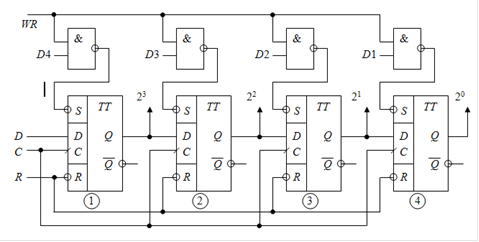
\includegraphics[width=\linewidth]{49}\\
Режим работы схемы:\\
\begin{enumerate}
  \item Сдвиг =0\\
  ПЧ = 0\\
  Уст в 0 = 0\\
  $Q_i = 0$ \\
  \item Сдвиг =0\\
  ПЧ = 1\\
  Уст в 0 = 1\\
  $Q_i = x_i$\\
  \item Сдвиг =1\\
  ПЧ = 0\\
  Уст в 0 = 1\\
  $Q_{i+1} = Q_i$ Информация запишется в 1 ступень последующего триггера
\end{enumerate}

Направление сдвига определяется коммутацией входов и выходов соответсвующих разрядов. $x_i$ -прием последующего кода.\\
Необходимо использовать двуступеньчатый триггер или триггер с динамическим управлением записью. Одноступеньчатые со статическим управлением записью - НЕЛЬЗЯ.
Так как во время действия синхросигнала изменяется состояние выходов триггеров.
Поскольку  эти триггеры подключены ко входам последующих триггеров , то за время действия синхросигнала измениться состояние и последующих триггеров,
следовательно информация в регистре сдвинется более чем на 1 разряд за 1 такт, следовательно не будет нормального функционирования.\\
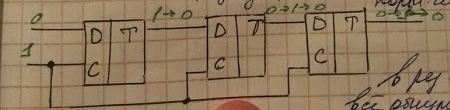
\includegraphics[width=\linewidth]{50}\\
В результате все обнулиться.

Прием информации в 2 направлениях\\
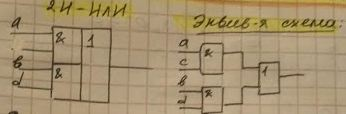
\includegraphics{51}\\
$f  = ac + bd $\\
$
\begin{cases}
c = 1\\
d = 0\\
\end{cases}
f = a\\
\begin{cases}
c = 0\\
d = 1\\
\end{cases}
f = b
$

\textbf{Реверсивные сдвигающие регистры}\\
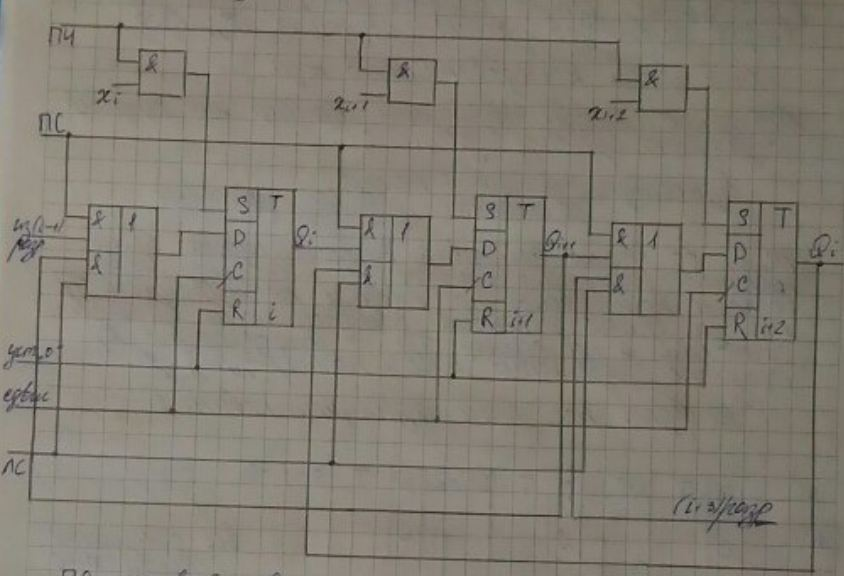
\includegraphics[width=\linewidth]{60}\\
ПС - правый сдвиг.\\
ЛС - левый сдвиг.\\
$
\begin{cases}
\text{ПС} = 1\\
\text{ЛС} = 0\\
\text{Сдвиг} = 1
\end{cases}
Q_{i+1} = Q_i\\
\begin{cases}
\text{ПС} = 0\\
\text{ЛС} = 1\\
\text{Сдвиг} = 1
\end{cases}
Q_{i+1} = Q_{i+2}\\
$\\
$
\begin{cases}
\text{ПС} = 0\\
\text{ЛС} = 0\\
\end{cases}
Q_{i+1} = 0\\
\begin{cases}
\text{ПС} = 1\\
\text{ЛС} = 1\\
\end{cases}
\text{Запрещенное состояние}\\
$\\
\textbf{Преобразование последовательного кода числа в паралелльный}\\
Последовательный в паралелльный\\
 Путем **** последовательного кода и его параллельной выдаче.\\
Параллельный в последовательный \\
 Используется параллельный прием (ПЧ = 1) и последовательная выдача кода с помощью операции сдвига.\\

УГО РЕГИСТРОВ\\
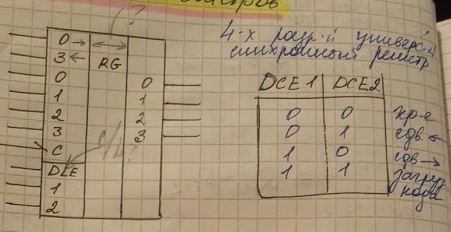
\includegraphics{61}\\

\newpage
\textbf{Класисификация счетчиков}
\begin{enumerate}
  \item По направлению счёта
  \begin{itemize}
    \item Суммирующие
    \item Вычитающие
    \item Реверсивные
  \end{itemize}
  \item По коэффициенту счёта
  \begin{itemize}
    \item Двоичные
    \item Двоично-десятичные (декадные)
    \item С другим модулем счёта
  \end{itemize}
  \item По способу организации внутренних связей
  \begin{itemize}
    \item С последовательным переносом
    \item С параллельным переносом
    \item Со сквозным переносом
    \item С групповым переносом
  \end{itemize}
  \item По порядку изменения состояния
  \begin{itemize}
    \item С естественным порядком счета
    \item С произвольным порядком счета
  \end{itemize}
  \item По способу переключения
  \begin{itemize}
    \item Асинхронные
    \item Синхронные
    \begin{itemize}
      \item Однотактные
      \item Двухтактные
    \end{itemize}
  \end{itemize}
\end{enumerate}

В асинхронных счетчиках переключения состояний происходит
в момент поступления управляющего сигнала.

В синхронных - по синхронному сигналу при наличии управляющих сигналов.
